\documentclass[]{article}
\usepackage{geometry}   % my added package "geometry"
\geometry{letterpaper,tmargin=1in,bmargin=1in,lmargin=2.2cm,rmargin=2.2cm}
\usepackage[colorlinks,bookmarksopen,bookmarksnumbered,
citecolor=green,urlcolor=red]{hyperref}
\hypersetup{pdfauthor={Name}}
%%%%%%%%%%%%%%%%%%%%%%%%%%%%%%%%%%%%%%%%%%%%%%%%%%%%%%%%%%%%%%%%%%%%%%%%%
%\usepackage{graphicx}
\usepackage{graphics}
\usepackage{subcaption}
\usepackage{epsfig}
\usepackage{epstopdf}
\usepackage{amsfonts}
\usepackage{amssymb}
\usepackage{booktabs}
\usepackage{color,soul}
%%%%%%%%%%%%%%%%%%%%%%%%%%%%%%%%%%%%%%%%%%%%%%%%%%%%%%%%%%%%%%%%%
\usepackage{amsmath}
\usepackage{cleveref}
%\usepackage[fleqn]{amsmath}
\usepackage{lineno}
\usepackage{tikz}
\usepackage{standalone}
\usetikzlibrary{calc,patterns,arrows.meta,shapes.arrows,intersections,positioning}
\usetikzlibrary{decorations.pathmorphing,backgrounds,fit,petri}
\usepackage[percent]{overpic}
%%%%%%%%%%%%%%%%%%%%%%%%%%%%%%%%%%%%%%%%%%%%%%%%%%%%%%%%%%%%%%%%%
\usepackage{xcolor}
\usepackage{listings}
\lstset { %
	language=C++,
	backgroundcolor=\color{blue!5}, % set backgroundcolor
	basicstyle=\footnotesize\color{black},% basic font settingbasicstyle=\ttfamily\color{black}
	keywordstyle=\color{red},
	commentstyle=\color{violet},
	stringstyle=\color{blue},
	xleftmargin=2em,
	frame=single,
	framexleftmargin=2em,
	numbers=left,
	numberstyle=\tiny,
	numbersep=8pt,
}
%%%%%%%%%%%%%%%%%%%%%%%%%%%%%%%%%%%%%%%%%%%%%%%%%%%%%%%%%%%%%%%%%
\renewcommand\thesubsection{\thesection\Alph{subsection}}
%%%%%%%%%%%%%%%%%%%%%%%%%%%%%%%%%%%%%%%%%%%%%%%%%%%%%%%%%%%%%%%%%
%opening
\begin{document}
\title{HiperLife Tutorial: PoissonSurfaceNeumann}
\author{LaCàN}
\maketitle

\linenumbers
\section{Introduction} \label{sec: Int}
\subsubsection{Problem Definition} \label{sec: pd} 
The Poisson equation is the canonical elliptic PDE. For a domain $\Omega \subset \mathbb{R}^n$ with boundary $\partial \Omega$, the Poisson equation is like:
\begin{equation}\label{eq1}
	\begin{aligned}
		 -\Delta U =f \quad  \text{in } \Omega \\
		 \nabla U \cdot n = g  \quad  \text{on }  \partial \Omega
	\end{aligned}
\end{equation}
Here, $f$ and $g$ are input data which in this case we assume that $f = 1$ and $g=x_{2}\cos{(3\pi x_{1})}$, and $n$ denotes the normal vector of boundary.
\subsubsection{Boundary Condition} \label{sec: B.C}
We have used Neumann Condition along the lines $x_{2}=0$, and $x_{1}=1$, as depicted in Figure \ref{fig_SB}.

\begin{figure}[htbp]
	\centering
	
\documentclass[preprint,12pt,a4]{standalone}
\usepackage{geometry}   % my added package "geometry"
\geometry{letterpaper,tmargin=1in,bmargin=1in,lmargin=2.5cm,rmargin=2.5cm}
\usepackage{tikz}
\usetikzlibrary{calc,patterns,arrows.meta,shapes.arrows,intersections,positioning}
\usetikzlibrary{decorations.pathmorphing,backgrounds,fit,petri}
\usepackage{standalone}
\begin{document}
	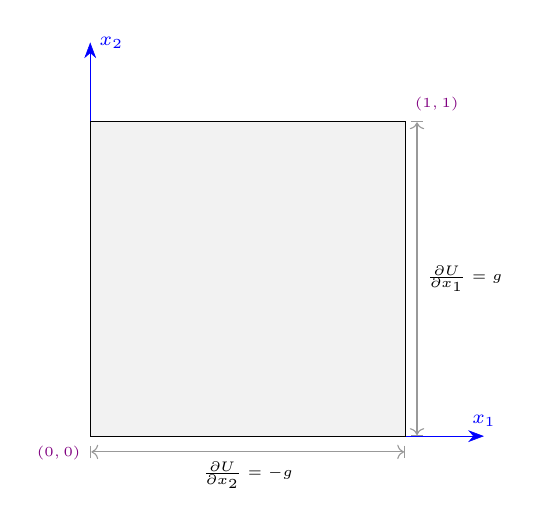
\begin{tikzpicture} [{place/.style={rectangle,draw=blue!50,fill=blue!20,ultra thin,inner sep=0.8mm}},{place2/.style={circle,draw=black!50,ultra thin,inner sep=0.8mm}},{linest/.style={color=gray,ultra thin}}]
	%%coordinates of corners of Beam
	\coordinate (A) at (0.0, 0.0);
	\coordinate (B) at (4.0, 0.0);
	\coordinate (C) at (4.0, 4.0);
	\coordinate (D) at (0.0, 4.0);
	%%axes
	\draw [{Stealth[length=2mm]}-{Stealth[length=2mm]}, help lines,blue] (5,0)node[above,font=\scriptsize]{$x_{1}$} -- (0,0) -- (0,5)node[right,font=\scriptsize] {$x_{2}$};
	%%square
	\draw [fill=gray!10] (A)node[font=\tiny, violet,below left]{$(0,0)$} rectangle  (C)node[font=\tiny, violet,above right]{$(1,1)$};
	
	%\draw [color=black](A)node[font=\tiny, violet,below left]{$(0,0)$} -- (A) -- (B)  -- %(C)node[font=\tiny, violet,above right]{$(1,1)$} -- (D) -- (A);
	%%B.C
	\draw [|<->|,gray!80]($(A)+(0,-0.2)$) --($(B)+(0,-0.2)$) node[fill=white,midway,below, font=\tiny,text=black] {$\frac{\partial{U}}{\partial{x_{2}}} =-g$};
	
	\draw [|<->|,gray!80]($(B)+(0.15,0.0)$)--($(C)+(0.15,0.0)$) node [fill=white,midway, right, font=\tiny, text=black] {$\frac{\partial{U}}{\partial{x_{1}}} =g$};
	\end{tikzpicture}
\end{document}
	\caption{Illustration of Geometry in $\Omega =[0,1]\times[0,1]$ and Boundary conditions on $\partial \Omega$.}
	\label{fig_SB}
\end{figure}

\section{Formulation} \label{sec: frml}
\subsubsection{Weak Form} \label{sec: WF}
To establish the weak form of Eq. (\ref{eq1}), it is multiplied with a weight-function, $w(x_1, x_2)$ to obtain
\begin{equation}\label{eq2}
	\begin{aligned}[b]
		-w\nabla^2 U &= wf \quad  \text{in }  \Omega \\
		w\nabla U \cdot n &= wg  \quad  \text{on }  \partial \Omega
	\end{aligned}
\end{equation}
By integrating this expression over $\Omega$, we have

\begin{equation}\label{eq3}
	\begin{aligned}[b]
		-\int_\Omega w\nabla^2 U = \int_\Omega wf
	\end{aligned}
\end{equation}
We know from calculus that $\nabla(w\nabla U) = \nabla w \cdot \nabla U + w\nabla ^2 U$. So we can write
\begin{equation}\label{eq4}
	\begin{aligned}[b]
		-\int_\Omega w\nabla^2U =  \int_{\Omega} \nabla w \cdot \nabla U - \int_{\Omega} \nabla(w\nabla U)
	\end{aligned}
\end{equation}
according to Gauss’s theorem
\begin{equation}\label{eq5}
	\begin{aligned}[b]
		\int_\Omega \nabla(w\nabla U)dA = \int_{\delta\Omega} w \nabla U \cdot n dS
	\end{aligned}
\end{equation}
by applying Eq. (\ref{eq5}) to Eq. (\ref{eq4})
\begin{equation}\label{eq6}
	\begin{aligned}[b]
		-\int_\Omega w\nabla^2U = \int_{\Omega} \nabla w \cdot \nabla U - \int_{\delta\Omega} w \nabla U \cdot n dS
	\end{aligned}
\end{equation}
the right-hand side of the Eq. (\ref{eq5}) is the second part of Eq. (\ref{eq2}), So now we can rewrite the Eq. (\ref{eq4}) like this
\begin{equation}\label{eq7}
	\begin{aligned}[b]
		 \int_{\Omega} \nabla w \cdot \nabla U dA = \int_\Omega wf dA + \int_{\partial \Omega} wg dS
	\end{aligned}
\end{equation}
\subsubsection{Basis Function} \label{sec: Basis Func}
We need to define basis functions for our 2D-domain and by it we can give an approximation of U.
\begin{equation}\label{eq8}
	\begin{aligned}[b]
		U(x,y) =\sum_{i=1}^{n} u_{i}\phi_{i}(x_{1},x_{2})
	\end{aligned}
\end{equation}
by applying Galerkin method the weight function is the same as basis function.
\begin{equation}\label{eq9}
	\begin{aligned}[b]
		w_{i} =\phi_{i}
	\end{aligned}
\end{equation}
in isoparametric concept even geometry is interpolated by same function. so
\begin{equation}\label{eq10}
	\begin{aligned}[b]
		X(x_{1},x_{2}) =\sum_{i=1}^{n} x_{i}\phi_{i}(x_{1},x_{2})
	\end{aligned}
\end{equation}
\subsubsection{Element} \label{sec: elem}
Triangular Element is used for discretization of bulk in this example, as shown in Fig. \ref{fig:sfig1}, 


The quadratic element consists of $9$ nodes would have interpolation functions for geometry and field variables like this. Let $\phi_{I}=N_I $ at element $T$.
\begin{equation}\label{eq11}
	\begin{aligned}[b]
		  N_{1}(\xi, \eta)  &= \xi(2\xi-1)
		& N_{2}(\xi, \eta)  &= 4\xi(1-\xi-\eta)\\
		%
		N_{3}(\xi, \eta)  &=    (1-\xi-\eta)(1-2\xi-2\eta)
		& N_{4}(\xi, \eta)  &=  4\xi\eta\\
		%
		N_{5}(\xi, \eta)  &= 4\eta(1-\xi-\eta)
		& N_{6}(\xi, \eta)  &= \eta(2\eta-1)
	\end{aligned}
\end{equation}

For the purpose of discretization of the boder in this example, 3-node line element is used, as shown in Fig. \ref{fig:sfig2}. which its interpolation functions would be like this.

\begin{figure}
	\begin{subfigure}{.5\textwidth}
		\centering
		\documentclass[preprint,12pt,a4]{standalone}
\usepackage{geometry}   % my added package "geometry"
\geometry{letterpaper,tmargin=1in,bmargin=1in,lmargin=2.5cm,rmargin=2.5cm}
\usepackage{tikz}
\usetikzlibrary{calc,patterns,arrows.meta,shapes.arrows,intersections,positioning}
\usetikzlibrary{decorations.pathmorphing,backgrounds,fit,petri}
\usepackage{standalone}
%
\begin{document}
	\begin{tikzpicture} [{place/.style={rectangle,draw=blue!50,fill=blue!20,ultra thin,inner sep=0.8mm}},{place2/.style={circle,draw=black!50,ultra thin,inner sep=0.8mm}},{linest/.style={color=gray,ultra thin}}]
		%axes
		\draw [{Stealth[length=2mm]}-{Stealth[length=2mm]}, help lines,blue] (5,0)node[above,font=\scriptsize]{$\xi$} -- (0,0) -- (0,5)node[right,font=\scriptsize] {$\eta$};
		%%element Nodes
		\node at (0.0,0.0) [place] (1) {};
		\node at (2.0,0.0) [place] (2) {};
		\node at (4.0,0.0) [place] (3) {};
		\node at (0.0,2.0) [place] (4) {};
		\node at (2.0,2.0) [place] (5) {};
		\node at (0.0,4.0) [place] (6) {};
		
		%\node at (0.66, 0.66) [place2] {};
		%\node at (2.66, 0.66) [place2] {};
		%\node at (0.66, 2.66) [place2] {};

		%%element border
		\draw [-] (1)node[below,font=\scriptsize]{$3$} --(2)node[below,font=\scriptsize]{$2$}--(3)node[below,font=\scriptsize]{$1$}--(5)node[right,font=\scriptsize]{$4$}--(6)node[right,font=\scriptsize]{$6$}--(4)node[left,font=\scriptsize]{$5$}--(1);
	\end{tikzpicture}
\end{document}
		\caption{}
		\label{fig:sfig1}
	\end{subfigure}%
	\begin{subfigure}{.5\textwidth}
		\centering
		\documentclass[preprint,12pt,a4]{standalone}
\usepackage{geometry}   % my added package "geometry"
\geometry{letterpaper,tmargin=1in,bmargin=1in,lmargin=2.5cm,rmargin=2.5cm}
\usepackage{tikz}
\usetikzlibrary{calc,patterns,arrows.meta,shapes.arrows,intersections,positioning}
\usetikzlibrary{decorations.pathmorphing,backgrounds,fit,petri}
\usepackage{standalone}
%
\begin{document}
	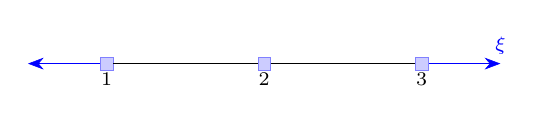
\begin{tikzpicture} [{place/.style={rectangle,draw=blue!50,fill=blue!20,ultra thin,inner sep=0.8mm}},{place2/.style={circle,draw=black!50,ultra thin,inner sep=0.8mm}},{linest/.style={color=gray,ultra thin}}]
		%axes
		\draw [{Stealth[length=2mm]}-{Stealth[length=2mm]}, help lines,blue] (5,0)node[above,font=\scriptsize]{$\xi$} -- (0,0)--(-1,0);
		%%element Nodes
		\node at (0.0,0.0) [place] (1) {};
		\node at (2.0,0.0) [place] (2) {};
		\node at (4.0,0.0) [place] (3) {};
		

		%%element border
		\draw [-] (1)node[below,font=\scriptsize]{$1$} --(2)node[below,font=\scriptsize]{$2$}--(3)node[below,font=\scriptsize]{$3$};
	\end{tikzpicture}
\end{document}
		\caption{}
		%\includegraphics[width=.8\linewidth]{image2}
		\label{fig:sfig2}
	\end{subfigure}
	\caption{ Schematic of the (a) bulk element (b) border element}
	\label{fig:elmnt}
\end{figure}


\begin{equation}\label{eq12}
	\begin{aligned}[b]
		N_{1}(\xi, \eta)  &=\frac{1}{2} \xi(\xi-1)
		& N_{2}(\xi, \eta)  &= 4\xi(1-\xi^2)
		& N_{3}(\xi, \eta)  &= \frac{1}{2} \xi(\xi+1)
	\end{aligned}
\end{equation}
\subsubsection{Elemental Integral} \label{sec: elem int}
  We want to compute the integral at Eq. (\ref{eq7}) over the element $T$
\begin{equation}\label{eq13}
	\begin{aligned}[b]
		\int_{\Omega_{T}} (\frac{\partial N_I}{\partial x_{1}}
		\frac{\partial N_J}{\partial x_{1}}+\frac{\partial N_I}{\partial x_{2}} 
		\frac{\partial N_J}{\partial x_{2}})U dA = \int_{\Omega_{T}} N_J f dA + \int_{\partial \Omega} N^{border}_J g dS
	\end{aligned}
\end{equation}
by the linear mapping between $(\xi,\eta)$ and $(x_{1},x_2)$, we can define $\frac{\partial N}{\partial x_{1}}$ and $\frac{\partial N}{\partial x_{2}}$
\begin{equation}\label{eq14}
	\begin{aligned}[b]
&
		\frac{\partial N}{\partial \xi} = \frac{\partial N}{\partial x_{1}}\frac{\partial x_{1}}{\partial \xi}+\frac{\partial N}{\partial x_{2}}\frac{\partial x_{2}}{\partial \eta}\\
& 
		\frac{\partial N}{\partial \eta} = \frac{\partial N}{\partial x_{1}}\frac{\partial x_{1}}{\partial \xi}+\frac{\partial N}{\partial x_{2}}\frac{\partial x_{2}}{\partial \eta}
	\end{aligned}
\end{equation}
Since $x=x(\xi,\eta)$, we get

\begin{equation}\label{eq15}
	\begin{aligned}[b]
		\begin{bmatrix}
			dx_{1}\\
			\\
			dx_{2}  
		\end{bmatrix}
		= \begin{bmatrix}
			\frac{\partial x_{1}}{\partial \xi}       & \frac{\partial x_{2}}{\partial \xi} \\
			\\
			\frac{\partial x_{1}}{\partial \eta}       &\frac{\partial x_{2}}{\partial \eta}\\
		\end{bmatrix}
		\begin{bmatrix}
			d \xi\\
			\\
			d \eta
		\end{bmatrix}
	\end{aligned}
\end{equation}
%
by defining Jacobian as
\begin{equation}\label{eq16}
	\begin{aligned}[b]
		J = \begin{bmatrix}
			\frac{\partial x_{1}}{\partial \xi}       & \frac{\partial x_{2}}{\partial \xi} \\
			\\
			\frac{\partial x_{1}}{\partial \eta}       &\frac{\partial x_{2}}{\partial \eta}\\
			\end{bmatrix}
	\end{aligned}
\end{equation}
so we can rewrite the Eq. (\ref{eq13}) 

\begin{equation}\label{eq17}
	\begin{aligned}[b]
\begin{bmatrix}
	\frac{\partial N}{\partial x_{1}}\\
	\\
	\frac{\partial N}{\partial x_{2}}  
\end{bmatrix}
= J^{-1}
\begin{bmatrix}
	\frac{\partial N}{\partial \xi}\\
	\\
	\frac{\partial N}{\partial \eta}
\end{bmatrix}
	\end{aligned}
\end{equation}
 by obtaining the terms Eq. (\ref{eq12}) now we can calculate the integral. So the elements of tangent matrix $K$ could be defined as
\begin{equation}\label{eq18}
	\begin{aligned}[b]
		K(i,j) = \int_{\Omega_{T}} (\frac{\partial N_{i}}{\partial x_{1}}
		\frac{\partial N_{j}}{\partial x_{1}}+\frac{\partial N_{i}}{\partial x_{2}} 
		\frac{\partial N_{j}}{\partial x_{2}}) dA
	\end{aligned}
\end{equation}
and for right-hand side
\begin{equation}\label{eq19}
	\begin{aligned}[b]
		F(i) = \int_{\Omega_{T}} N^{bulk}_{i}f dA + \int_{\partial \Omega} N^{border}_i g dS
	\end{aligned}
\end{equation}
Note that as it discussed earlier, different types of elements is used for bulk and border. At last we define $j$ as $j=det(J)$ because $dA=dx_{1} \times dx_{2}=jd\xi d\eta$.
\subsubsection{Integration method} \label{sec: int}
Let $f(\xi_{i},\eta_{i})=j(\frac{\partial N_{i}}{\partial x_{1}}
\frac{\partial N_{j}}{\partial x_{1}}+\frac{\partial N_{i}}{\partial x_{2}} 
\frac{\partial N_{j}}{\partial x_{2}})$, then by Gauss–Legendre quadrature we have
\begin{equation}\label{eq20}
	\begin{aligned}[b]
		\int_{-1}^1 \int_{-1}^1 f(\xi_{i},\eta_{i}) d\xi d\eta = \sum_{k=1}^{n}\sum_{l=1}^{m} \omega_{k}\omega_{l}f(\hat{\xi_{i}},\hat{\eta_{i}})
	\end{aligned}
\end{equation}
where $n$ and $m$ are the number of integration points used in each direction, $\omega$ is quadrature weights, $\hat{\xi_{i}}$ and $\hat{\eta_{i}}$ are the roots of the $n$th Legendre polynomial. In this example we use $3$ points integration as it shown in Fig. \ref{fig:ifig1}. $[W_{p}=\{\frac{1}{6}, \frac{1}{6},\frac{1}{6} \}, (\xi_{p}, \eta_{p})=\{(\frac{1}{6},\frac{1}{6}), (\frac{1}{6},\frac{2}{3}),  (\frac{2}{3},\frac{1}{6})\}]$.
\begin{figure}
	\begin{subfigure}{.5\textwidth}
		\centering
		\documentclass[preprint,12pt,a4]{standalone}
\usepackage{geometry}   % my added package "geometry"
\geometry{letterpaper,tmargin=1in,bmargin=1in,lmargin=2.5cm,rmargin=2.5cm}
\usepackage{tikz}
\usetikzlibrary{calc,patterns,arrows.meta,shapes.arrows,intersections,positioning}
\usetikzlibrary{decorations.pathmorphing,backgrounds,fit,petri}
\usepackage{standalone}
%
\begin{document}
	\begin{tikzpicture} [{place/.style={rectangle,draw=blue!50,fill=blue!20,ultra thin,inner sep=0.8mm}},{place2/.style={circle,draw=black!50,ultra thin,inner sep=0.8mm}},{linest/.style={color=gray,ultra thin}}]
		%axes
		\draw [{Stealth[length=2mm]}-{Stealth[length=2mm]}, help lines,blue] (4.5,0)node[above,font=\scriptsize]{$\xi$} -- (0,0) -- (0,4.5)node[right,font=\scriptsize] {$\eta$};
		%%element Nodes
		\node at (0.0,0.0) [place,fill=white] (1) {};
		\node at (2.0,0.0) [place,fill=white] (2) {};
		\node at (4.0,0.0) [place,fill=white] (3) {};
		\node at (0.0,2.0) [place,fill=white] (4) {};
		\node at (2.0,2.0) [place,fill=white] (5) {};
		\node at (0.0,4.0) [place,fill=white] (6) {};
		
		\node at (0.66, 0.66) [place2,fill=black!60] {};
		\node at (2.66, 0.66) [place2,fill=black!60] {};
		\node at (0.66, 2.66) [place2,fill=black!60] {};

		%%element border
		\draw [-] (1) -- (2) -- (3) -- (5) -- (6) -- (4) -- (1);
	\end{tikzpicture}
\end{document}
		\caption{}
		\label{fig:ifig1}
	\end{subfigure}%
	\begin{subfigure}{.5\textwidth}
		\centering
		\documentclass[preprint,12pt,a4]{standalone}
\usepackage{geometry}   % my added package "geometry"
\geometry{letterpaper,tmargin=1in,bmargin=1in,lmargin=2.5cm,rmargin=2.5cm}
\usepackage{tikz}
\usetikzlibrary{calc,patterns,arrows.meta,shapes.arrows,intersections,positioning}
\usetikzlibrary{decorations.pathmorphing,backgrounds,fit,petri}
\usepackage{standalone}
%
\begin{document}
	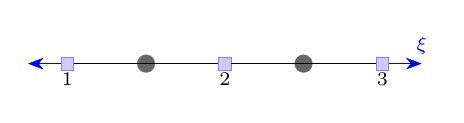
\begin{tikzpicture} [{place/.style={rectangle,draw=blue!50,fill=blue!20,ultra thin,inner sep=0.8mm}},{place2/.style={circle,draw=black!50,ultra thin,inner sep=0.8mm}},{linest/.style={color=gray,ultra thin}}]
		%axes
		\draw [{Stealth[length=2mm]}-{Stealth[length=2mm]}, help lines,blue] (2.5,0)node[above,font=\scriptsize]{$\xi$} -- (0,0)--(-2.5,0);
		%%element Nodes
		\node at (-2.0,0.0) [place] (1) {};
		\node at (0.0,0.0) [place] (2) {};
		\node at (2.0,0.0) [place] (3) {};
		
		\node at (-1, 0.0) [place2,fill=black!60] {};
		\node at (1, 0.0) [place2,fill=black!60] {};
		

		%%element border
		\draw [-] (1)node[below,font=\scriptsize]{$1$} --(2)node[below,font=\scriptsize]{$2$}--(3)node[below,font=\scriptsize]{$3$};
	\end{tikzpicture}
\end{document}
		\caption{}
		%\includegraphics[width=.8\linewidth]{image2}
		\label{fig:ifig2}
	\end{subfigure}
	\caption{(a) 2-D integration on Triangle element (b) 1-D integration on line element}
	\label{fig:int}
\end{figure}
At the border we use $2$ points integration as it shown in Fig. \ref{fig:ifig2}. $[W_{p}=1, \xi_{p}=\mp \frac{1}{\sqrt{3}}]$

\section{Implementation} \label{sec: imp}
In this section, we present implementation of our solution in the Hiperlife.
\nolinenumbers
\subsubsection{Headers} \label{sec: hdr}
\begin{lstlisting}
#include <iostream>
#include <fstream>
#include "hl_Core.h"
#include "hl_ParamStructure.h"
#include "hl_Parser.h"
#include "hl_TypeDefs.h"
#include "hl_MeshLoader.h"
#include "hl_StructMeshGenerator.h"
#include "hl_DistributedMesh.h"
#include "hl_FillStructure.h"
#include "hl_DOFsHandler.h"
#include "hl_HiPerProblem.h"
#include "hl_SurfLagrParam.h"
#include "hl_LinearSolver_Iterative_AztecOO.h"
\end{lstlisting}

\subsubsection{Parameters} \label{sec: ppr}
\begin{lstlisting}
struct PoissonParams
{
	enum RealParameters
	{
		strength
	};
	
	enum StringParameters
	{
		filemesh
	};
	
	HL_PARAMETER_LIST DefaultValues{
		{"filemesh", ""},
		{"strength", 1.0},
	};
};
\end{lstlisting}

\subsubsection{Initializing} \label{sec: main}
\begin{lstlisting}
void LS(hiperlife::FillStructure& fillStr);
void RHS_Border(hiperlife::FillStructure& fillStr);

int main(int argc, char** argv)
{
	using namespace std;
	using namespace hiperlife;
\end{lstlisting}

\subsubsection{Defining parameters of the model} \label{sec: Pstr}
\begin{lstlisting}
	SmartPtr<ParamStructure> paramStr = ReadParamsFromCommandLine<PoissonParams>();
\end{lstlisting}

\subsubsection{Mesh Generation} \label{sec: mshG}
\begin{lstlisting}
	SmartPtr<StructMeshGenerator> mesh = Create<StructMeshGenerator>();
	mesh->setElemType(ElemType::Triang);
	mesh->setBasisFuncType(BasisFuncType::Lagrangian);
	mesh->setBasisFuncOrder(2);
	mesh->genSquare(4,1.0);
\end{lstlisting}

\subsubsection{Mesh Distribution} \label{sec: mshD}
\begin{lstlisting}
	SmartPtr<DistributedMesh> disMesh = Create<DistributedMesh>();
	disMesh->setMesh(mesh);
	disMesh->setBalanceMesh(true);
	disMesh->Update();
\end{lstlisting}

\subsubsection{DOFs Handler} \label{sec: dofC}
\begin{lstlisting}
	SmartPtr<DOFsHandler> dofHand = Create<DOFsHandler>(disMesh);
	dofHand->setNameTag("dofHand");
	dofHand->setNumDOFs(1);
	dofHand->setNumElemAuxF(1);
	dofHand->Update();
\end{lstlisting}

\subsubsection{Boundary conditions and Constraints} \label{sec: BC}
\begin{lstlisting}
	if (!disMesh->hasBorder())
	{
		if (disMesh->myRank() == 0)
		dofHand->setConstraint(0, 0, IndexType::Local, 0.0);
	}
	else
	{
		for (int i = 0; i < disMesh->loc_nPts(); i++)
		{
			if (disMesh->nodeCrease(i, IndexType::Local) > 0 and
			disMesh->nodeCoord(i, 1, IndexType::Local) > 0)
			dofHand->setConstraint(0,i,IndexType::Local, 0.0);
		}
	}
	dofHand->UpdateGhosts();
\end{lstlisting}

\subsubsection{HiperProblem} \label{sec: hpc}
\begin{lstlisting}
	SmartPtr<HiPerProblem> hiperProbl = Create<HiPerProblem>();
	
	hiperProbl->setParameterStructure(paramStr);
	hiperProbl->setDOFsHandlers({dofHand});
	
	hiperProbl->setIntegration("Integ", {"dofHand"});
	hiperProbl->setCubatureGauss("Integ",3);
	hiperProbl->setElementFillings("Integ", LS);
	
	hiperProbl->setIntegration("BorderInteg", {"dofHand"});
	hiperProbl->setCubatureBorderGauss("BorderInteg",2,{MAxis::Xmax,MAxis::Ymin});
	hiperProbl->setElementFillings("BorderInteg", nullptr, nullptr, RHS_Border);
	
	hiperProbl->setGlobalIntegrals({"BorderLength"});
	
	hiperProbl->Update();
\end{lstlisting}

\subsubsection{Solver Settings} \label{sec: slv}
\begin{lstlisting}
	SmartPtr<AztecOOIterativeLinearSolver> solver=Create<AztecOOIterativeLinearSolver>();
	solver->setHiPerProblem(hiperProbl);
	solver->setTolerance(1.E-8);
	solver->setMaxNumIterations(500);
	solver->setSolver(AztecOOIterativeLinearSolver::Solver::Gmres);
	solver->setPreconditioner(AztecOOIterativeLinearSolver::Preconditioner::Neumann);
	solver->setDefaultParameters();
	solver->setVerbosity(AztecOOIterativeLinearSolver::Verbosity::High);
	solver->Update();
	
	solver->solve();
	solver->UpdateSolution();
\end{lstlisting}

\subsubsection{Finalization and Postprocessing} \label{sec: fnl}
\begin{lstlisting}
	dofHand->printFileLegacyVtk("PoissonSurface");
	
	if (dofHand->myRank() == 0)
	cout<<std::scientific<<std::setprecision(5)<<"Border Length = "<<endl;
	cout<<hiperProbl->globalIntegral("BorderLength")<<endl;
	
	ofstream rhsFile;
	rhsFile.open(paramStr->getStringParameter(PoissonParams::filemesh)+
	to_string(dofHand->myRank())+".txt");
	hiperProbl->sol->Print(rhsFile);
	rhsFile.close();
	
	hiperlife::Finalize();
	return 0;
}
\end{lstlisting}

\subsubsection{Filling left-hand side matrix} \label{sec: lhs}
\begin{lstlisting}
void LS(hiperlife::FillStructure& fillStr)
{
	using namespace std;
	using namespace hiperlife;
	using hiperlife::Tensor::tensor;
	
	double strength = fillStr.getRealParameter(PoissonParams::strength);

	SubFillStructure& subFill = fillStr["dofHand"];
	int DOF  = subFill.numDOFs;
	int eNN  = subFill.eNN;
	int nDim = subFill.nDim;
	int pDim = subFill.pDim;
	vector<double>& nborCoords  = subFill.nborCoords;
	
	double* bf  = subFill.nborBFs();
	double* dbf_l = subFill.nborBFsGrads();	
	double x[3]={};
	for (int i = 0; i < eNN; i++) // i from 0 to 5
	{
		for (int n = 0; n < nDim; n++) // n from 0 to 2
		{
			x[n] += nborCoords[i*nDim+n] * bf[i];
		}
	}
	
	double g_cc[4]={};
	double xu[3]={};
	double xv[3]={};
	SurfLagrParam::MetricTensor(g_cc, xu, xv, eNN, nborCoords.data(), dbf_l);
	
	double g_CC[4]={};
	Math::Invert2x2(g_CC, g_cc);
	
	double jac = sqrt(Math::DetMat2x2(g_cc));
	
	double source = strength * x[1]*cos(3.0*M_PI*x[0]);
	
	for (int i = 0; i < eNN; i++)
	{
		double* dbf_lI_c = &dbf_l[pDim*i];
		
		double dbf_lI_C[2]={};
		Math::MatProduct(dbf_lI_C, 2, 2, 1, g_CC, dbf_lI_c);
		
		for (int j = 0; j < eNN; j++)
		{
			double* dbf_lJ_c = &dbf_l[pDim*j];
			
			fillStr.Ak(0,0)[i*DOF*eNN+j*DOF] += jac*Math::Dot2D(dbf_lI_C,dbf_lJ_c);
		}
		
		fillStr.Bk(0)[i*DOF] += jac * bf[i] * source;
	}
	
	return;
}
\end{lstlisting}

\subsubsection{Filling right-hand side vector} \label{sec: rhs}
\begin{lstlisting}
void RHS_Border(hiperlife::FillStructure& fillStr)
{
	using namespace std;
	using namespace hiperlife;
	using hiperlife::Tensor::tensor;

	SubFillStructure& subFill = fillStr["dofHand"];
	int DOF  = subFill.numDOFs;
	int eNN  = subFill.eNN; 
	int nDim = subFill.nDim;
	vector<double>& nborCoords = subFill.nborCoords;
	double *bf  = subFill.nborBFs();
	double *dbf_l = subFill.nborBFsGrads();
	
	double Ip[4], xu[3], xv[3];
	SurfLagrParam::MetricTensor(Ip, xu, xv, eNN, nborCoords.data(), dbf_l);
	
	auto bTangentRef = subFill.tangentsBoundaryRef();
	double bTangent[3]={};
	for (int n = 0; n < nDim; n++)
	bTangent[n] = bTangentRef[0] * xu[n] + bTangentRef[1]*xv[n];
	double jac = Math::Norm3D(bTangent);
	
	for (int i = 0; i < eNN; i++)
	fillStr.Bk(0)[i*DOF] += jac*bf[i];
	
	fillStr.addToGlobalIntegral("BorderLength", jac);
}
\end{lstlisting}
\section{Results} \label{sec: rst}
\begin{figure}[htbp]
	\centering
	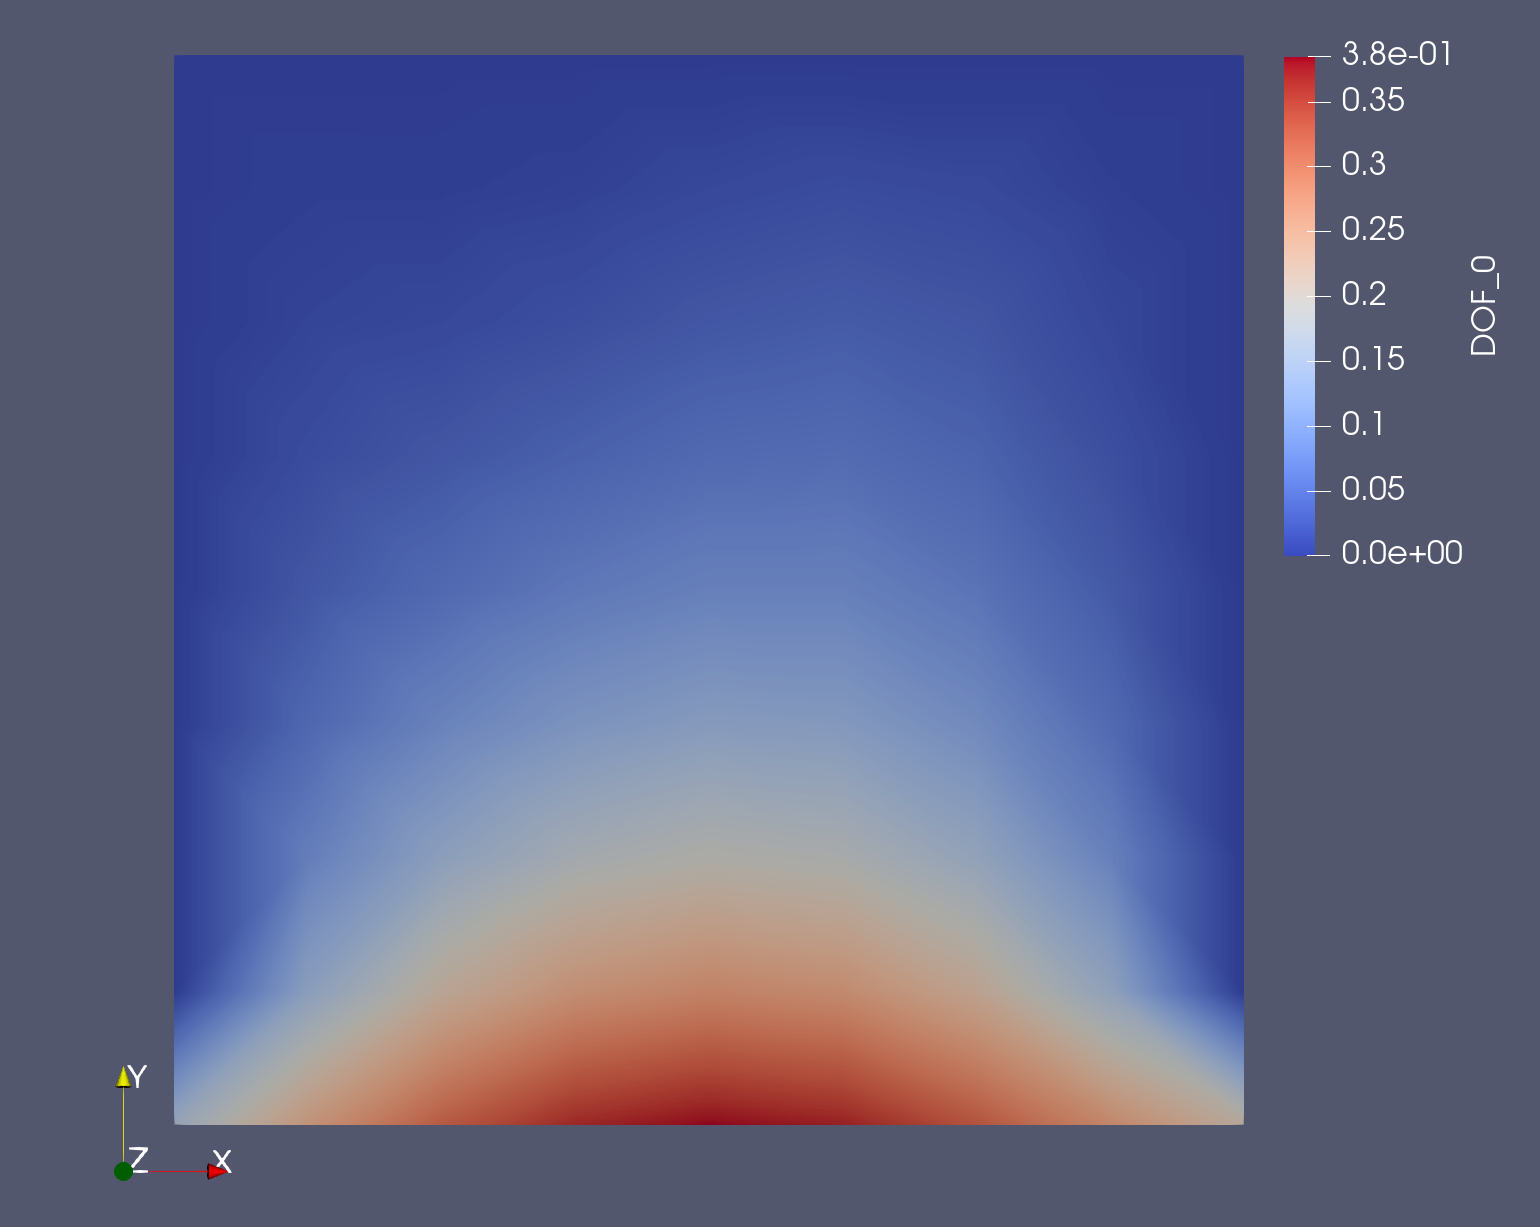
\includegraphics[width=0.5\textwidth]{Figures/result.png}
	\caption{Solution.}
	\label{fig_rst}
\end{figure}
\pagebreak
\section*{Appendix} \label{sec: apx}
\end{document}
